\documentclass[margin=0mm,tikz]{standalone}

\usepackage{tikz}
\usepackage{xcolor}
%\usepackage{mathtools}
%\usepackage{stackengine}

\usetikzlibrary{positioning}
\usetikzlibrary{fit}
\usetikzlibrary{calc}
\usetikzlibrary{arrows.meta}
\usetikzlibrary{quotes}
\usetikzlibrary{backgrounds}

\pgfdeclarelayer{background}
\pgfsetlayers{background,main}

% -----------------------
% colors
% -----------------------
\definecolor{conv1color}{RGB}{175, 0, 23}
\definecolor{conv3color}{RGB}{255, 0, 10}
\definecolor{convblockcolor}{RGB}{0, 93, 157}
\definecolor{downscalecolor}{RGB}{113, 0, 162}
\definecolor{upscalecolor}{RGB}{0, 138, 5}
\definecolor{forwardcolor}{RGB}{100, 100, 100}
\definecolor{skipcolor}{RGB}{218, 138, 0}
\definecolor{operatorcolor}{RGB}{136, 150, 186}
\definecolor{reccolor}{RGB}{150, 150, 20}


% Set background color
%\pagecolor{white}

% -----------------------
% colors
% -----------------------


\tikzstyle{mt-node} = [
    thick, 
    draw=fluxkernelcolor!50!gray,
    top color = fluxkernelcolor!20!white,
    bottom color = fluxkernelcolor!30!white,
    rounded corners,
    minimum size=1.5cm
]

\tikzstyle{nn-node} = [
    thick, 
    %circle,
    rounded corners=0.5mm,
    draw, 
    text width=6.5mm,
    align=center,
    text=black, 
    top color = nncolor!20!white,
    bottom color =nncolor!30!white,
    minimum size=1.0cm, 
    inner sep=0pt
]

\tikzstyle{operator} = [
    circle,
    draw,
    top color = skipcolor!70!white,
    bottom color = skipcolor!80!white, 
    text=black,
    minimum size=0.5cm,
    inner sep=0pt
]

\tikzstyle{finndashed} = [dash pattern=on 2pt off 1.5pt]

\tikzstyle{conv1} = [-{Latex[length=6pt, width=10pt]}, line width=3pt, conv1color]
\tikzstyle{conv3} = [-{Latex[length=6pt, width=10pt]}, line width=3pt, conv3color]
\tikzstyle{convblock} = [-{Latex[length=6pt, width=10pt]}, line width=3pt, convblockcolor]
\tikzstyle{downscale} = [-{Latex[length=6pt, width=10pt]}, line width=3pt, downscalecolor]
\tikzstyle{upscale} = [-{Latex[length=6pt, width=10pt]}, line width=3pt, upscalecolor]
\tikzstyle{forward} = [-{Latex[length=2pt, width=4pt]}, line width=1pt, forwardcolor]
\tikzstyle{skip} = [-{Latex[length=3pt, width=5pt]}, line width=2pt, skipcolor]
\tikzstyle{rec} = [-{Latex[length=6pt, width=10pt]}, line width=3pt, reccolor]


\tikzset{
	annotated cuboid/.pic={
		\tikzset{%
			every edge quotes/.append style={midway, auto},
			/cuboid/.cd,
			#1
		}

		% coordinate scheme of the cube
		%
		%    e---------h
		%   /|        /|
		%  / |       / |
		% a---------d  |
		% |  |      |  |
		% |  f------|--g
		% | /       | /
		% |/        |/
		% b---------c
		
		% Set up the corner coordinates of the cube
		\coordinate (a) at (-\cwidth*\cscale*0.5, \cheight*\cscale*0.5, 0);
		\coordinate (b) at (-\cwidth*\cscale*0.5, -\cheight*\cscale*0.5, 0);
		\coordinate (c) at (\cwidth*\cscale*0.5, -\cheight*\cscale*0.5, 0);
		\coordinate (d) at (\cwidth*\cscale*0.5, \cheight*\cscale*0.5, 0);
		\coordinate (e) at (-\cwidth*\cscale*0.5, \cheight*\cscale*0.5, -\cdepth*\cscale);
		\coordinate (f) at (-\cwidth*\cscale*0.5, -\cheight*\cscale*0.5, -\cdepth*\cscale);
		\coordinate (g) at (\cwidth*\cscale*0.5, -\cheight*\cscale*0.5, -\cdepth*\cscale);
		\coordinate (h) at (\cwidth*\cscale*0.5, \cheight*\cscale*0.5, -\cdepth*\cscale);
		

		% Clip the cube image to the outer coordinates
		\clip (a) -- (b) -- (c) -- (g) -- (h) -- (e) -- cycle;
		
		%
		% Draw the cube
		
		% Dashed, hidden lines
		\draw[\ccolor, dashed, very thick] (f) -- (b);
		\draw[\ccolor, dashed, very thick] (f) -- (g);
		\draw[\ccolor, dashed, very thick] (f) -- (e);
		
		% Faces
		\draw[fill=\ccolor, opacity=0.6] (a) -- (b) -- (c) -- (d) -- cycle;  % front
		\draw[fill=\ccolor, opacity=0.6] (a) -- (d) -- (h) -- (e) -- cycle;  % top
		\draw[fill=\ccolor, opacity=0.6] (d) -- (c) -- (g) -- (h) -- cycle;  % right
		
		% Redraw edges of the faces
		\draw[\ccolor, very thick] (a) -- (b) -- (c) -- (d) -- cycle;  % front
		\draw[\ccolor, very thick] (a) -- (d) -- (h) -- (e) -- cycle;  % top
		\draw[\ccolor, very thick] (d) -- (c) -- (g) -- (h) -- cycle;  % right
		
		% Draw annotations
		\draw (a) edge ["\textbf{\lheight}"] (b);
		\draw (b) edge ["\textbf{\lwidth}"] (c);
	
		% Define the node for this kernel
		\node [anchor=north west, minimum width=\cwidth*\cscale cm, minimum height=\cheight*\cscale cm] (\clabel) at (a) {};
	
	},
	/cuboid/.search also={/tikz},
	/cuboid/.cd,
	width/.store in=\cwidth,
	height/.store in=\cheight,
	depth/.store in=\cdepth,
	units/.store in=\cunits,
	scale/.store in=\cscale,
	label/.store in=\clabel,
	lwidth/.store in=\lwidth,
	lheight/.store in=\lheight,
	ccolor/.store in=\ccolor,
	width=1,
	height=1,
	depth=1,
	units=cm,
	scale=1.0,
	label=dummy,
	lwidth=2,
	lheight=2,
	ccolor=gray,
}

\begin{document}
	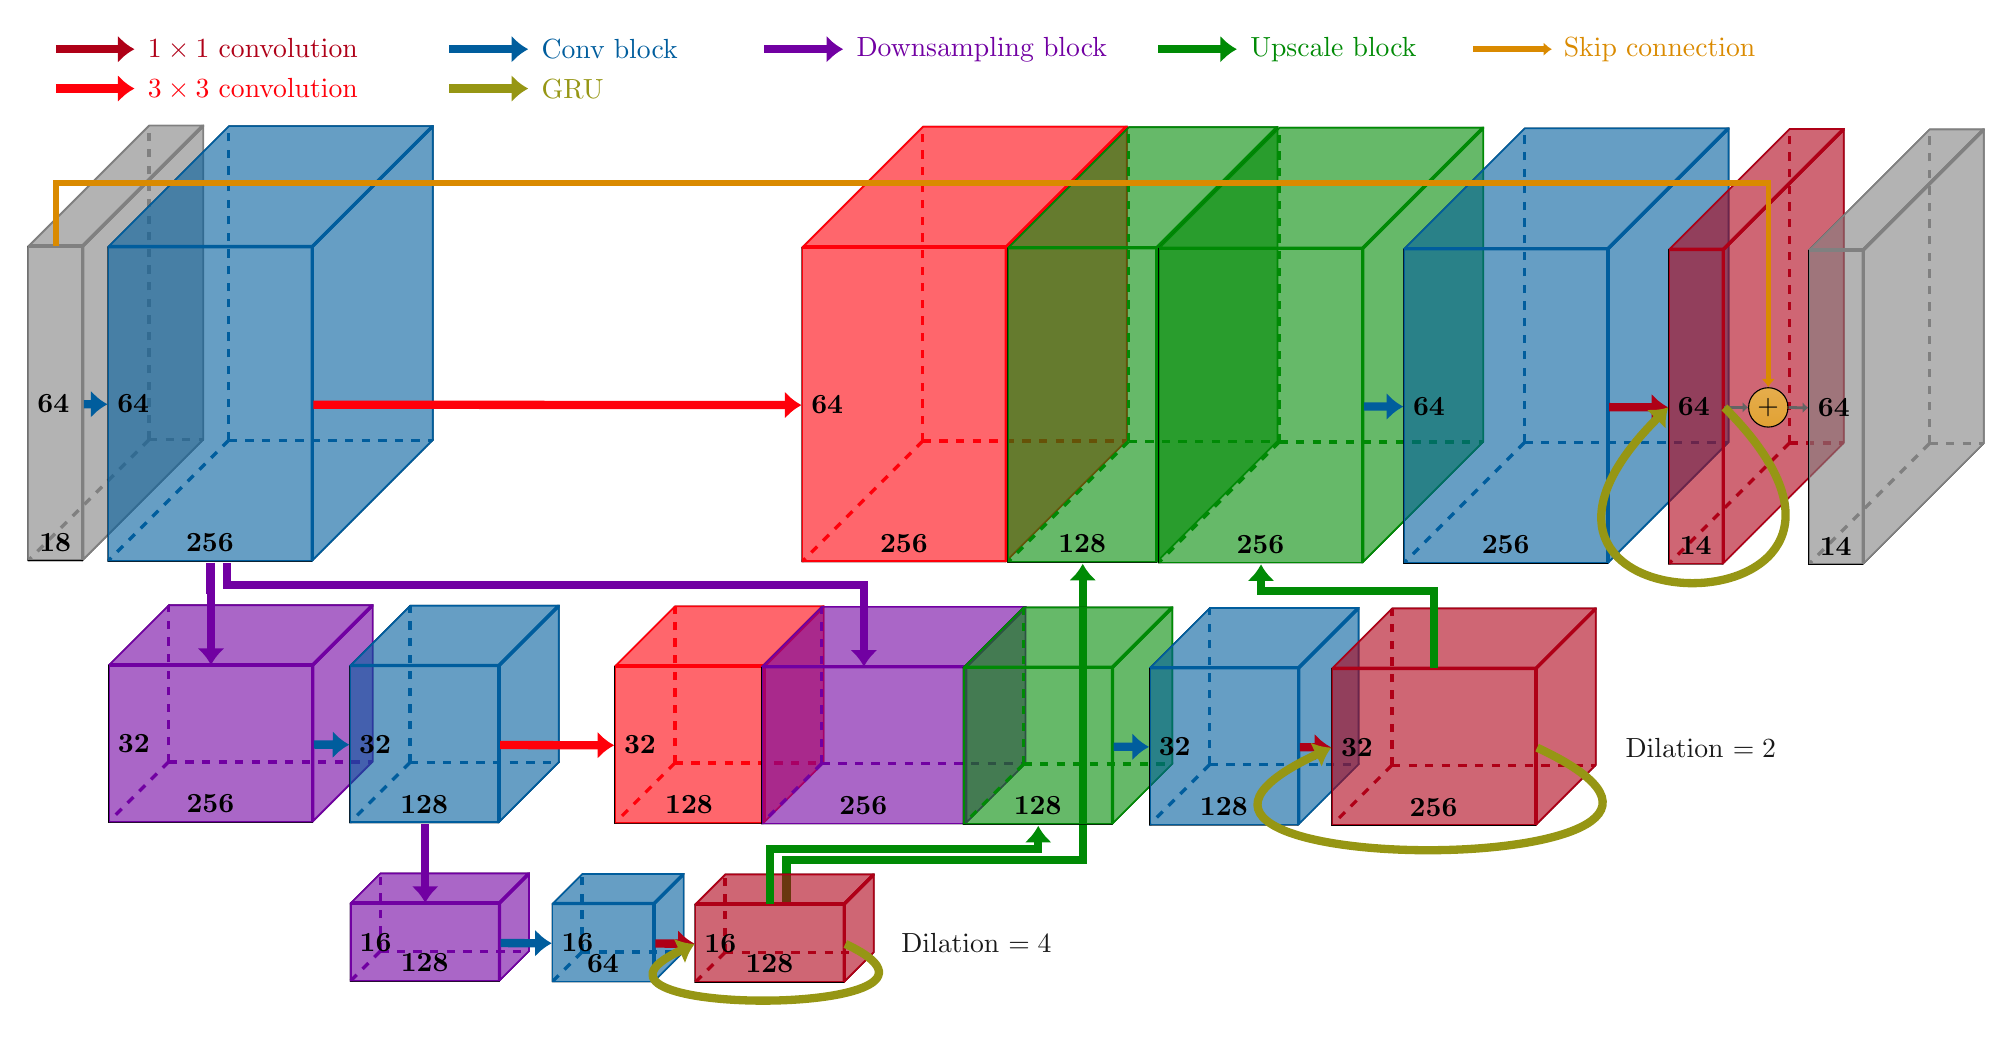
\begin{tikzpicture}
	
	%
	% First layer down
	
	% Maps
	\pic {annotated cuboid={width=0.7, height=4, depth=4, units=, label=input, lwidth=18, lheight=64}};
	\pic [right=1.6cm of input] {annotated cuboid={width=2.6, height=4, depth=4, units=, label=e1-1, lwidth=256, lheight=64, ccolor=convblockcolor}};
	
	% Arrows
	\draw[convblock] (input) -- (e1-1);
	
	%
	% Second layer down
	
	% Maps
	\pic [below=2.3cm of e1-1] {annotated cuboid={width=2.6, height=2, depth=2, units=, label=e2-1, lwidth=256, lheight=32, ccolor=downscalecolor}};
	\pic [right=1.4cm of e2-1] {annotated cuboid={width=1.9, height=2, depth=2, units=, label=e2-2, lwidth=128, lheight=32, ccolor=convblockcolor}};
	
	% Arrows
	\draw[downscale] (e1-1.south) --++ (0, -10pt) -- ([yshift=-10pt]e1-1.south -| e2-1.north) -- (e2-1.north);
	\draw[convblock] (e2-1) -- (e2-2);
	
	%
	% Third layer down (synoptic layer)
	
	% Maps
	\pic [below=1.5cm of e2-2] {annotated cuboid={width=1.9, height=1, depth=1, units=, label=e3-1, lwidth=128, lheight=16, ccolor=downscalecolor}};
	\pic [right=1.3cm of e3-1] {annotated cuboid={width=1.3, height=1, depth=1, units=, label=e3-2, lwidth=64, lheight=16, ccolor=convblockcolor}};
	\pic [right=1.45cm of e3-2] {annotated cuboid={width=1.9, height=1, depth=1, units=, label=e3-3, lwidth=128, lheight=16, ccolor=conv1color}};
	
	% Arrows
	\draw[downscale] (e2-2.south) --++ (0, -10pt) -- ([yshift=-10pt]e2-2.south -| e3-1.north) -- (e3-1.north);
	\draw[convblock] (e3-1) -- (e3-2);
	\draw[conv1] (e3-2) -- (e3-3);
	\draw[rec] (e3-3.east) to [out=-25, in=-155, looseness=3] (e3-3.west);
	
	% Dilation remark
	\node[right=3cm of e3-2, gray!20!black] {Dilation $= 4$};
	
	% Second layer up
	
	% Maps
	\pic [right=2.4cm of e2-2] {annotated cuboid={width=1.9, height=2, depth=2, units=, label=d2-1, lwidth=128, lheight=32, ccolor=conv3color}};
	\pic [right=1.25cm of d2-1] {annotated cuboid={width=2.6, height=2, depth=2, units=, label=d2-2, lwidth=256, lheight=, ccolor=downscalecolor}};
	\pic [right=0.9cm of d2-2] {annotated cuboid={width=1.9, height=2, depth=2, units=, label=d2-3, lwidth=128, lheight=, ccolor=upscalecolor}};
	\pic [right=1.4 of d2-3] {annotated cuboid={width=1.9, height=2, depth=2, units=, label=d2-4, lwidth=128, lheight=32, ccolor=convblockcolor}};
	\pic [right=1.7 of d2-4] {annotated cuboid={width=2.6, height=2, depth=2, units=, label=d2-5, lwidth=256, lheight=32, ccolor=conv1color}};
		
	% Arrows
	\draw[conv3] (e2-2) -- (d2-1);
	\draw[downscale] ([xshift=6pt]e1-1.south) --++ (0, -8pt) -- ([yshift=-8pt]e1-1.south -| d2-2.north) -- (d2-2.north);
	\draw[upscale] (e3-3.north) --++ (0, 20pt) -- ([yshift=20pt]e3-3.north -| d2-3.south) -- (d2-3.south);
	\draw[convblock] (d2-3) -- (d2-4);
	\draw[conv1] (d2-4) -- (d2-5);
	\draw[rec] (d2-5.east) to [out=-25, in=-155, looseness=4] (d2-5.west);
	
	% Dilation remark
	\node[right=1cm of d2-5, gray!20!black] {Dilation $= 2$};
	
	%
	% First layer up
	
	\pic [right=7.5cm of e1-1] {annotated cuboid={width=2.6, height=4, depth=4, units=, label=d1-1, lwidth=256, lheight=64, ccolor=conv3color}};
	\pic [right=0.95cm of d1-1] {annotated cuboid={width=1.9, height=4, depth=4, units=, label=d1-2, lwidth=128, lheight=, ccolor=upscalecolor}};
	\pic [right=1.3cm of d1-2] {annotated cuboid={width=2.6, height=4, depth=4, units=, label=d1-3, lwidth=256, lheight=, ccolor=upscalecolor}};
	\pic [right=1.8 of d1-3] {annotated cuboid={width=2.6, height=4, depth=4, units=, label=d1-4, lwidth=256, lheight=64, ccolor=convblockcolor}};
	\pic [right=1.1 of d1-4] {annotated cuboid={width=0.7, height=4, depth=4, units=, label=d1-5, lwidth=14, lheight=64, ccolor=conv1color}};
	\node[operator, right=0.3 of d1-5] (plus1) {$+$};
	\pic [right=0.6 of plus1] {annotated cuboid={width=0.7, height=4, depth=4, units=, label=d1-6, lwidth=14, lheight=64}};

	% Arrows
	\draw[conv3] (e1-1) -- (d1-1);
	\begin{scope}[on background layer]
		\draw[upscale] ([xshift=6pt]e3-3.north) --++ (0, 16pt) -- ([yshift=16pt]e3-3.north -| d1-2.south) -- (d1-2.south);
	\end{scope}
	\draw[upscale] (d2-5.north) --++ (0, 28pt) -- ([yshift=28pt]d2-5.north -| d1-3.south) -- (d1-3.south);
	\draw[convblock] (d1-3) -- (d1-4);
	\draw[conv1] (d1-4) -- (d1-5);
	\draw[forward] (d1-5) -- (plus1);
	\draw[skip] (input.north) --++ (0, 0.8cm) -- ([yshift=0.8cm]input.north -| plus1.north) -- (plus1.north);
	\draw[forward] (plus1) -- (d1-6);
	\draw[rec] (d1-5.east) to [out=-45, in=-135, looseness=15] (d1-5.west);
	
	%
	% Legend
	\draw[conv1] ([yshift=2.5cm]input.north) --++ (1, 0) node[right] (conv1label) {$1\times1$ convolution};
	\draw[conv3] ([yshift=2.0cm]input.north) --++ (1, 0) node[right] (conv3label) {$3\times3$ convolution};
	\draw[convblock] ([yshift=2.5cm, xshift=5cm]input.north) --++ (1, 0) node[right] (convblocklabel) {Conv block};
	\draw[downscale] ([yshift=2.5cm, xshift=9cm]input.north) --++ (1, 0) node[right] (downscalelabel) {Downsampling block};
	\draw[upscale]([yshift=2.5cm, xshift=14cm]input.north) --++ (1, 0) node[right] (upscalelabel) {Upscale block};
	\draw[skip] ([yshift=2.5cm, xshift=18cm]input.north) --++ (1, 0) node[right] (skipcolor) {Skip connection};
	\draw[rec] ([yshift=2.0cm, xshift=5cm]input.north) --++ (1, 0) node[right] (reccolor) {GRU};
		
	\end{tikzpicture}
\end{document}